%%%%%%%%%%%%%%%%%%%%%%%%%%%%%%%%%%%%%%%%%%%%%%%%%%%%%%%%%%%%%
%%	Results													%
%%%%%%%%%%%%%%%%%%%%%%%%%%%%%%%%%%%%%%%%%%%%%%%%%%%%%%%%%%%%%

\section{Results}

%-----------------------------------------------------------
%	Model fit
%-----------------------------------------------------------
\subsection{Model fit and parameter estimation}



	Using $\Psi_{eff}$ (Eqn. \ref{eqn:finalexponentialmodelformscaled}) significantly improves the fit to the responses of the structural model (Eqn. \ref{eqn:fullcollagen}) with an average $R^2$ of 0.958 (n = 6). Specifically, the improvement is mainly in fitting the non-physiologic range, defined as the range away from the equi-biaxial strain region, specifically uniaxial strain or pure shear (Fig. \ref{fig:modelfit}). The time taken for parameter estimation (5-10 seconds) is also significantly lower in comparison to meso-scale structural approaches, such for the mitral valve \cite{zhang_meso_2016} (10-40 minutes) and exogenously crosslinked tissues \cite{zhang_modeling_2017}(30 min - 4 hours).
    
%%%%%%%%%%%%%%%%%%%%%%%%%%%%%%%%%%%%%%%%%%%%%%%%%%%%%%%%%%%%
%-------------------	begin FIGURE 	-------------------%
\begin{figure}
\centering
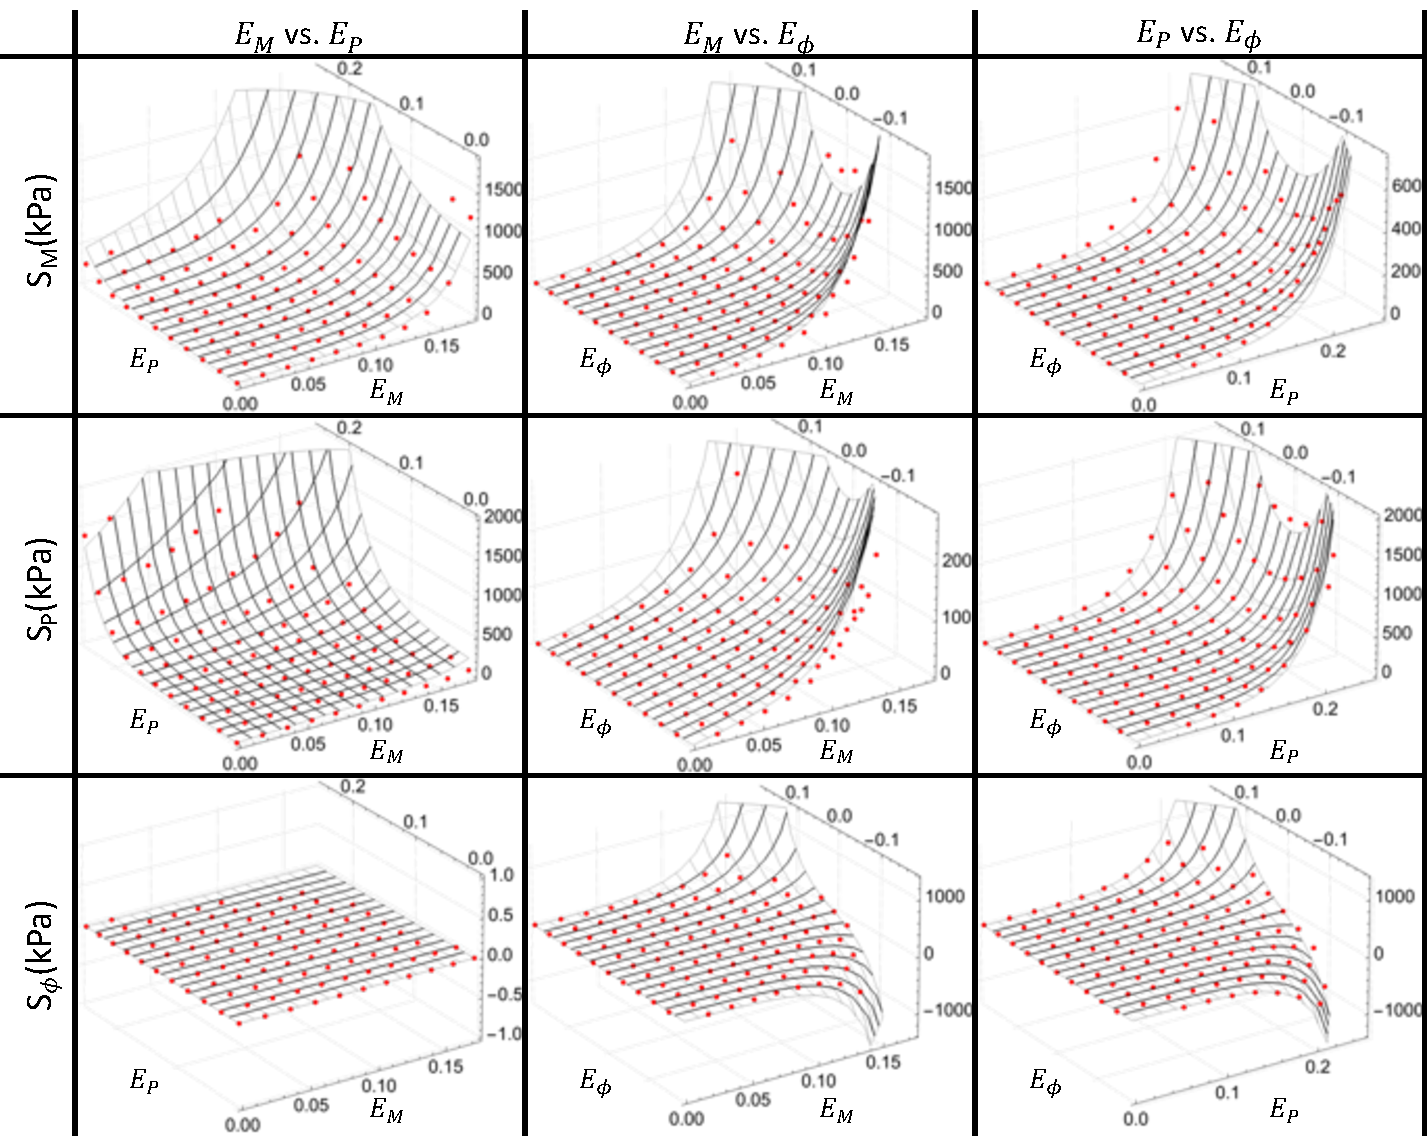
\includegraphics[width=6.5in]{Figures/modelfit}
\caption{Parameter estimation results showing that $\Psi_{eff}$ is able to match response function (Eqn. \ref{eqn:responsefunctions}) (Top) $S_m = \partial\Psi/\dif E_m$, (Middle) $S_n = \partial\Psi/\dif E_n$, and (Bottom) $S_\phi = \partial\Psi/\dif E_\phi$ for each pair of Green Lagrange strain components.}
\label{fig:modelfit}
\end{figure} 
%-------------------	 end FIGURE 	-------------------%
%%%%%%%%%%%%%%%%%%%%%%%%%%%%%%%%%%%%%%%%%%%%%%%%%%%%%%%%%%%%
    
%     Furthermore, we found that fitting the effective model to existing data sufficiently preserves the mechanical response of glutaraldehyde pericardium such that we were able to obtain similar structural model parameters in comparison to fitting to the structural model directly. There are some minor differences, especially in the modulus, but that is impart due to the fact that the experimental data is somewhat lacking, particularly in terms of examining the response of the material to shearing, but this is still enough for us to obtain reasonably accurate structural model parameters. The accuracy can be further improved if we import the microstructural of the material, the ODF and RDF, directly.  

% %----------------------------------------------------------%
% %-------------------	begin TABLE 	-------------------%
% \begin{table}
% \caption{Comparison between structural model parameters when fitting to the experimental data directly vs. to the effective constitutive model fitted to the experimental data. UB is the abbreviation for upper-bound.}
% \begin{center}
% \label{tb:inverseparameterestimation}
% \begin{tabular}{|l|p{40pt}|p{45pt} p{25pt} p{25pt} p{25pt} p{25pt} p{25pt}|p{60pt}|}
% \hline

%  	& \centering Matrix \mbox modulus (kPa)	
%     & \centering Collagen \mbox{modulus} (kPa)	
%     & \centering ODF mean $(\deg)$	
%     & \centering ODF stdev	$(\deg)$ 
%     & {\centering $D(\lambda_s)$ mean}
%     & \centering $D(\lambda_s)$ stdev	
%     & {\centering $D(\lambda_s)$ UB}
%     & {\centering Interactions modulus (kPa)}\\
% \hline
% FSM to data	& 102.8	& 302	& 0	& 32.7	& 1.187	& 0.022	& 1.213	& 1785.7	\\
% \hline
% FSM to EMM	& 97.1	& 288	& 0	& 34.1	& 1.192	& 0.023 & 1.221	& 2085.3	\\
% \hline
% \end{tabular}
% \end{center}
% \end{table}
% %-------------------	 end TABLE 		-------------------%
% %----------------------------------------------------------%


%-----------------------------------------------------------
%	Parameter estimation convergence
%-----------------------------------------------------------
\subsection{Convergence}

	In addition, we found that the model scaling method is very effective. Parameters converges in approximately 40-60 iterations regardless of starting point, where are the algorithm can require 40-120 iterations without using scaling. This is of course due to the fact that the algorithm can be trapped within the valley region where the gradient is small, reducing the step size during search. Of course, with sufficiently good initial guess, both methods are essentially equivalent.



%-----------------------------------------------------------
%	Optimal experimental design
%-----------------------------------------------------------
\subsection{Optimal \textit{in silico} loading paths}

	Based on our results, the optimal loading paths for parameter estimation is rather intuitive. For a single loading path, this is the equi-biaxial stress loading path. D-optimality is several hundred times higher for the equi-biaxial stress loading path in comparison to all other loading paths, i.e. the D-optimality for other loading paths are nearly zero. Even so the D-optimality is still on the order of $10^{-17}$, implying that a single loading path is not sufficient to determine the model parameters of highly non-linear hyperelastic tissues. The type of stress is not explicitly listed, rather this depends on the choice of objective function, i.e. if the parameter estimation is done using the difference in second Piola Kirchhoff stress then the choice of the loading path should be equi-biaxial in second Piola Kirchhoff stress. 
    
    
%%%%%%%%%%%%%%%%%%%%%%%%%%%%%%%%%%%%%%%%%%%%%%%%%%%%%%%%%%%%
%-------------------	begin FIGURE 	-------------------%
\begin{figure}[hbtp]
\centering
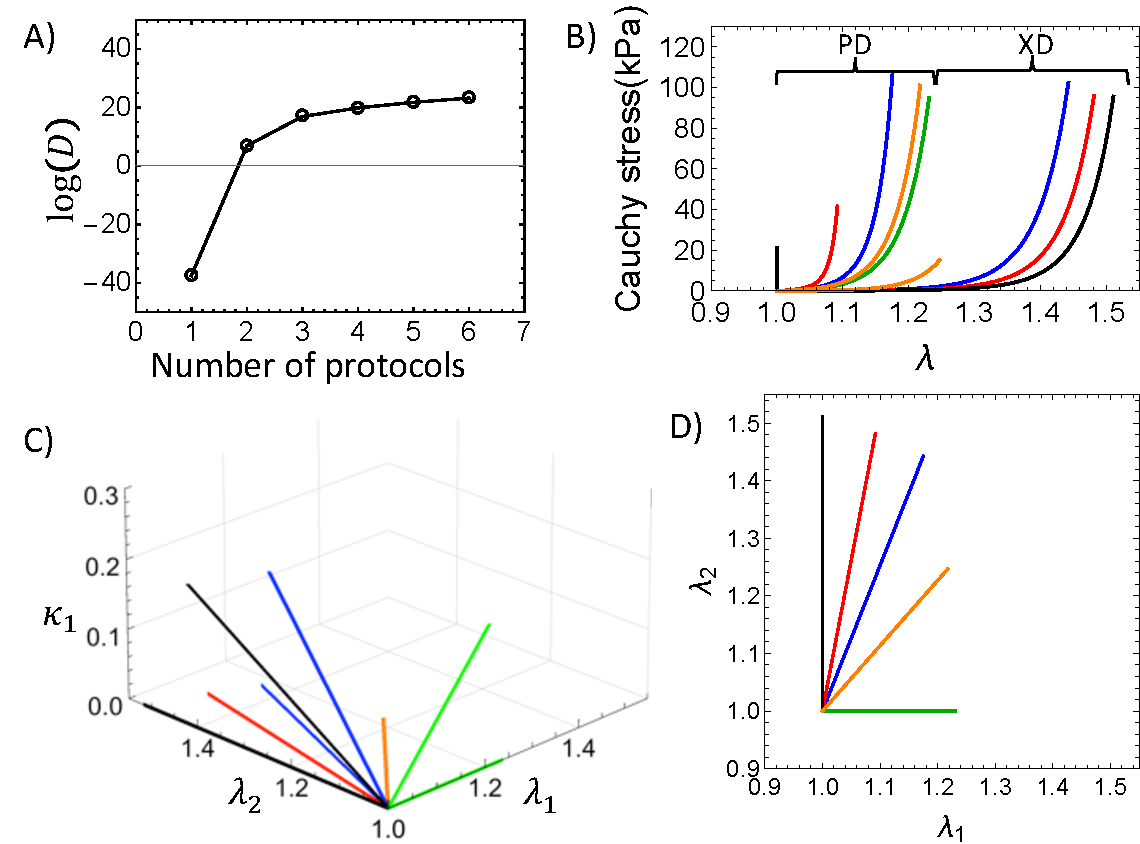
\includegraphics[width=5.5in]{Figures/doptimality}
\caption{A) The best D-optimality value for a given number of loading paths used to generate the data, which stops increasing significantly after three. B) The stress-strain curve of the optimal set of five loading paths with no shear. C) The full set of optimal loading paths including the shear component are shown. The same colored loading paths are built upon the corresponding D) planar stretch loading paths by adding a shear component. }
\label{fig:doptimality}
\end{figure} 
%-------------------	 end FIGURE 	-------------------%
%%%%%%%%%%%%%%%%%%%%%%%%%%%%%%%%%%%%%%%%%%%%%%%%%%%%%%%%%%%%

    
    The value of D-optimality significantly improved with the addition of a second loading path, increasing from $5.2 \times 10^{-17}$ to $9.7 \times 10^2$, nearly 20 orders in magnitude. Using three loading paths leads to another significant increase to $2.2 \times 10^7$, 5 orders of magnitude. Further additional loading paths only improve the D-optimality by 1 order of magnitude, where the D-optimality is $4.2 \times 10^8$, $2.8 \times 10^9$ and $1.2 \times 10^{10}$ for four, five and sixth loading paths respectively. It can be said that three is the minimal number of loading paths necessary for parameter estimation. Indeed, for dense collagenous soft tissues this appears to be true. In practice, it's better to add a few additional loading paths as a precaution. For this reason, using five loading paths is more preferred (Fig. \ref{fig:doptimality}D). The reason why four loading paths is not chosen is because the specific loading paths are not consistent and maybe even model dependent if it is even (see Appendix \ref{sec:optimalpaths}, Fig. \ref{fig:evenpaths}). For odd number of loading paths, these are the equibiaxial stress, the boundaries of the range of interest, and the average ratios in between (see Appendix \ref{sec:optimalpaths}, Fig. \ref{fig:oddpaths}). With the addition of shear, we found this to be the minimal three loading paths adding to it a shear component up to the maximum value (Fig. \ref{fig:doptimality}C). Further addition does not change the D-optimality by any significant quantity. More detailed results are presented in Appendix \ref{sec:optimalpaths}.
    
    
  
% phy1 norm = 1.35315
% phy3 norm = 19834.0


   

%-----------------------------------------------------------
%	Vs Fung
%-----------------------------------------------------------
\subsection{Reproducing soft tissue response}

	For the Sun \textit{et al.} \cite{sun_biaxial_2003} study, the generalized Fung model (Eqn. \ref{eqn:generalizedfungmodela}) fitted the five loading paths in the physiologic range very well (Fig. \ref{fig:fungphyfit}), but predicted the remaining unfitted loading paths poorly (Fig. \ref{fig:fungphypred}). Similarly, when the non-physiologic loading paths are fit ((Fig. \ref{fig:fungphyfit})), the remaining protocols are still predicted poorly. However, we do note here that the generalized Fung model cannot fit the non-physiologic protocols very well. This is as expected since the generalized Fung model can only approximate the response of soft tissues in a limited range (Section \ref{sec:possibleforms}). 

%%%%%%%%%%%%%%%%%%%%%%%%%%%%%%%%%%%%%%%%%%%%%%%%%%%%%%%%%%%%
%-------------------	begin FIGURE 	-------------------%
\begin{figure}[hptb]
\centering
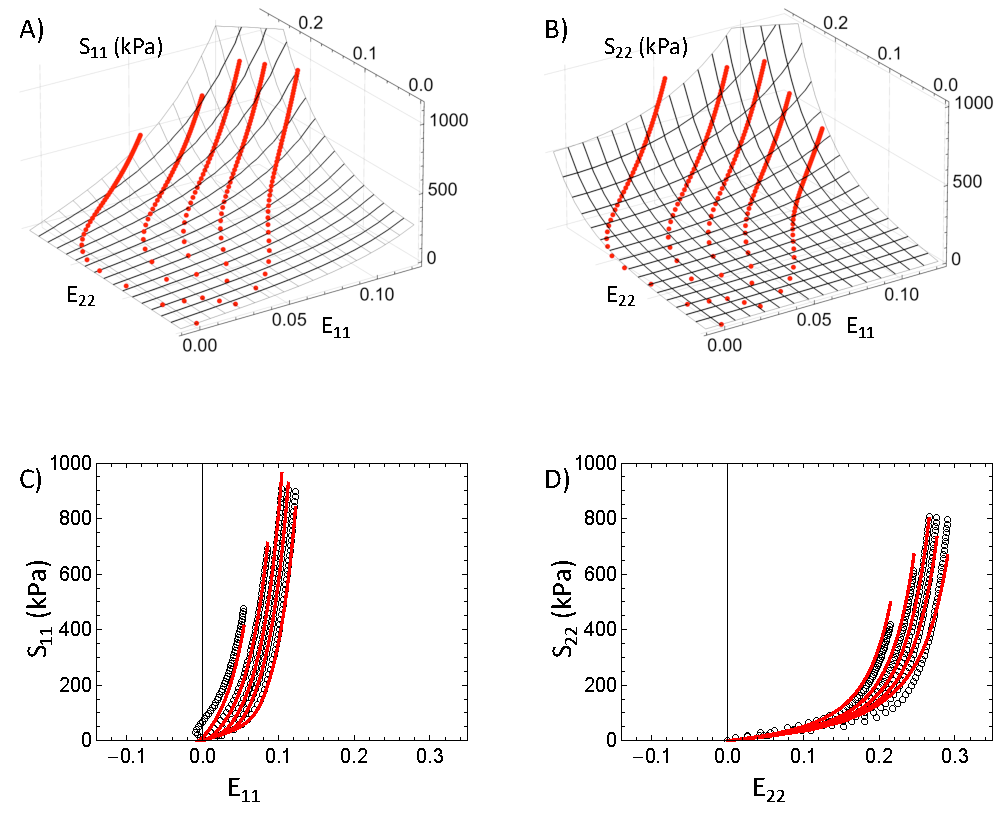
\includegraphics[width=6.5in]{Figures/fungphyfit}
\caption{Reproducing the results of Sun \textit{et al.} \cite{sun_biaxial_2003} showing that the generalized Fung model is able to fit the loading paths in the physiologic range very well. A) The $S_{11}$ surface. B) The $S_{22}$ surface. C) Best fit of the $S_{11}$ component of the loading paths. D) Best fit of the $S_{22}$ component of the loading paths.}
\label{fig:fungphyfit}
\end{figure} 
%-------------------	 end FIGURE 	-------------------%
%%%%%%%%%%%%%%%%%%%%%%%%%%%%%%%%%%%%%%%%%%%%%%%%%%%%%%%%%%%%

%%%%%%%%%%%%%%%%%%%%%%%%%%%%%%%%%%%%%%%%%%%%%%%%%%%%%%%%%%%%
%-------------------	begin FIGURE 	-------------------%
\begin{figure}[hptb]
\centering
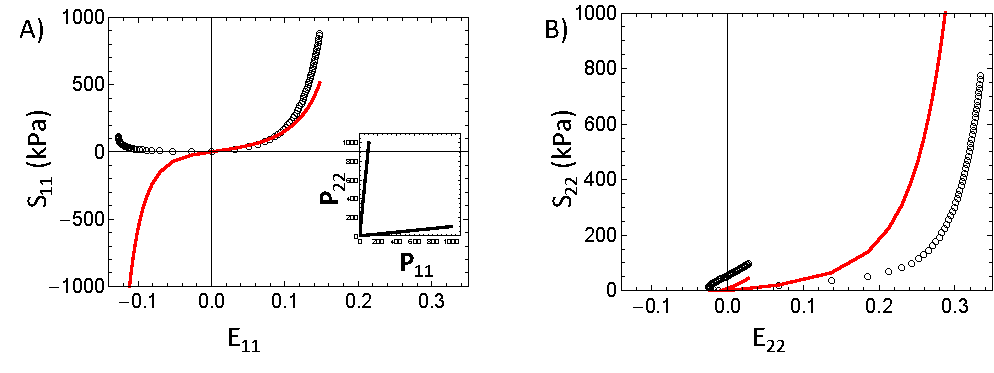
\includegraphics[width=6.5in]{Figures/fungphypred}
\caption{Reproducing the results of Sun \textit{et al.} \cite{sun_biaxial_2003} showing the A) $S_{11}$ component and B) $S_{22}$ component of the remaining unfitted loading paths are predicted poorly from fit (Fig. \ref{fig:fungphyfit}). The inset in A shows the corresponding loading paths.}
\label{fig:fungphypred}
\end{figure} 
%-------------------	 end FIGURE 	-------------------%
%%%%%%%%%%%%%%%%%%%%%%%%%%%%%%%%%%%%%%%%%%%%%%%%%%%%%%%%%%%%


%%%%%%%%%%%%%%%%%%%%%%%%%%%%%%%%%%%%%%%%%%%%%%%%%%%%%%%%%%%%
%-------------------	begin FIGURE 	-------------------%
\begin{figure}[hptb]
\centering
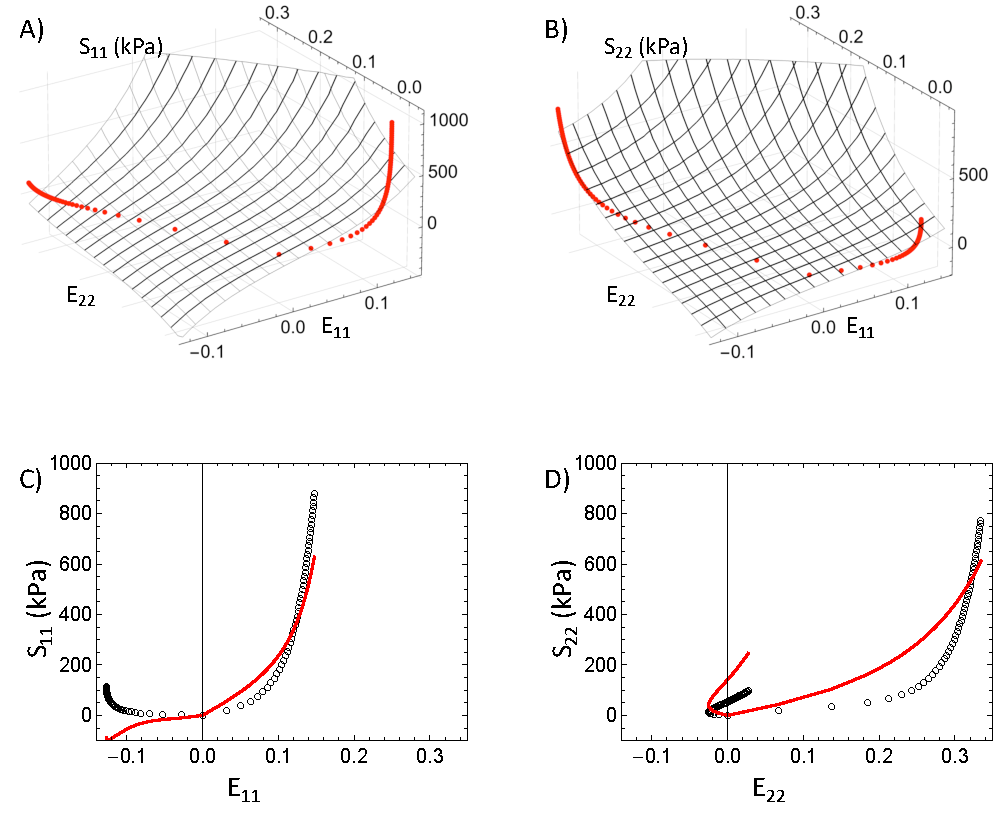
\includegraphics[width=6.5in]{Figures/fungoutfit}
\caption{Reproducing the results of Sun \textit{et al.} \cite{sun_biaxial_2003} showing the best fit of the generalized Fung model to the loading paths in the non-physiologic range is poor. A) The $S_{11}$ surface. B) The $S_{22}$ surface. C) Best fit of the $S_{11}$ component of the loading paths. D) Best fit of the $S_{22}$ component of the loading paths.}
\label{fig:fungoutfit}
\end{figure} 
%-------------------	 end FIGURE 	-------------------%
%%%%%%%%%%%%%%%%%%%%%%%%%%%%%%%%%%%%%%%%%%%%%%%%%%%%%%%%%%%%

%%%%%%%%%%%%%%%%%%%%%%%%%%%%%%%%%%%%%%%%%%%%%%%%%%%%%%%%%%%%
%-------------------	begin FIGURE 	-------------------%
\begin{figure}[hptb]
\centering
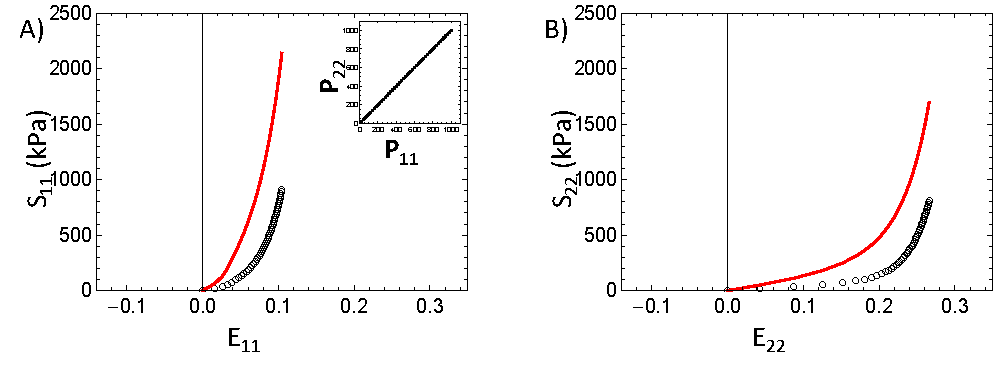
\includegraphics[width=6.5in]{Figures/fungoutpred}
\caption{Reproducing the results of Sun \textit{et al.} \cite{sun_biaxial_2003} showing the A) $S_{11}$ component and B) $S_{22}$ component of the equi-biaxial stress loading path are predicted poorly from fit (Fig. \ref{fig:fungoutfit}). The inset in A shows the corresponding loading paths.}
\label{fig:fungoutpred}
\end{figure} 
%-------------------	 end FIGURE 	-------------------%
%%%%%%%%%%%%%%%%%%%%%%%%%%%%%%%%%%%%%%%%%%%%%%%%%%%%%%%%%%%%
    

    
    

    
    
    
% %%%%%%%%%%%%%%%%%%%%%%%%%%%%%%%%%%%%%%%%%%%%%%%%%%%%%%%%%%%%
% %-------------------	begin FIGURE 	-------------------%
% \begin{figure}[!hbtp]
% \centering
% \includegraphics[width=4.5in]{Figures/sunreproduce}
% \caption{Reproducing the fit of the generalized Fung model to A) the loading paths in the physiologic range (range most likely to contain the physiologic loading path) and B) the non-physiologic loading paths in Sun \textit{et al.} \cite{sun_biaxial_2003}}
% \label{fig:sunreproduce}
% \end{figure} 
% %-------------------	 end FIGURE 	-------------------%
% %%%%%%%%%%%%%%%%%%%%%%%%%%%%%%%%%%%%%%%%%%%%%%%%%%%%%%%%%%%%

% %%%%%%%%%%%%%%%%%%%%%%%%%%%%%%%%%%%%%%%%%%%%%%%%%%%%%%%%%%%%
% %-------------------	begin FIGURE 	-------------------%
% \begin{figure}[!hbtp]
% \centering
% \includegraphics[width=6.5in]{Figures/sunstresses}
% \caption{Reproducing the resulting stress strain behavior of 1) the fitted response and 2) the prediction of the remaining loading paths of the generalized Fung model to A) the loading paths in the physiologic range and B) the non-physiologic loading paths in Sun \textit{et al.} \cite{sun_biaxial_2003}}
% \label{fig:sunstresses}
% \end{figure} 
% %-------------------	 end FIGURE 	-------------------%
% %%%%%%%%%%%%%%%%%%%%%%%%%%%%%%%%%%%%%%%%%%%%%%%%%%%%%%%%%%%%

% %%%%%%%%%%%%%%%%%%%%%%%%%%%%%%%%%%%%%%%%%%%%%%%%%%%%%%%%%%%%
% %-------------------	begin FIGURE 	-------------------%
% \begin{figure}[!hbtp]
% \centering
% \includegraphics[width=4.5in]{Figures/effectivereproduce}
% \caption{The response of fitting $\Psi_{eff}$ to A) minimal 3 optimal loading paths and B) the post pre-strain region define in Fung \textit{et al.} \cite{fung_pseudoelasticity_1979}}
% \label{fig:effectivereproduce}
% \end{figure} 
% %-------------------	 end FIGURE 	-------------------%
% %%%%%%%%%%%%%%%%%%%%%%%%%%%%%%%%%%%%%%%%%%%%%%%%%%%%%%%%%%%%
% %%%%%%%%%%%%%%%%%%%%%%%%%%%%%%%%%%%%%%%%%%%%%%%%%%%%%%%%%%%%
% %-------------------	begin FIGURE 	-------------------%
% \begin{figure}[!hbtp]
% \centering
% \includegraphics[width=6.5in]{Figures/effectivestresses}
% \caption{The stress strain behavior of 1) the fitted response and 2) the prediction of the other loading paths using $\Psi_{eff}$ to A) optimal loading paths and B) the physiologic or post pre-strain range only.}
% \label{fig:effectivestresses}
% \end{figure} 
% %-------------------	 end FIGURE 	-------------------%
% %%%%%%%%%%%%%%%%%%%%%%%%%%%%%%%%%%%%%%%%%%%%%%%%%%%%%%%%%%%%

    
	Although the quality of fit is improved with $\Psi_{eff}$ (Eqn. \ref{eqn:finalexponentialmodelformscaled}) (Fig. \ref{fig:effphyfit}), using non-optimal loading paths, such as based on Fung \textit{et al.}'s post-pre-strain protocols \cite{fung_pseudoelasticity_1979}, lead to poor predictions for other loading paths (Fig. \ref{fig:effphypred}). Although not obvious at first, $\Psi_{eff}$ severe underestimates the response of the material in the low stress region. The D-optimality with two protocols in this post-pre-strain range is only $1.35$, which improves to $1.98\times 10^4$ with six protocols. This pales in comparison to in comparison to with $9.7 \times 10^2$ for the two optimal protocols and $2.2 \times 10^7$ with three optimal protocols. When both $\Psi_{eff}$ and three optimal loading paths are utilized, we find that the loading paths are both fitted (Fig. \ref{fig:effoptfit}) and predicted very well (Fig. \ref{fig:effoptpred}). We also testing other non-optimal loading paths with minor modifications to the form of $\Psi_{eff}$ (Appendix \ref{sec:otherresults}). To briefly summarize, without an optimal set of loading paths, $\Psi_{eff}$ is not able to fully predict out side of the fitted range. When this happens, the form of $\Psi_{eff}$ can have unpredictable impact on the predicted response, even though the quality of fit are very similar. 


%%%%%%%%%%%%%%%%%%%%%%%%%%%%%%%%%%%%%%%%%%%%%%%%%%%%%%%%%%%%
%-------------------	begin FIGURE 	-------------------%
\begin{figure}[hptb]
\centering
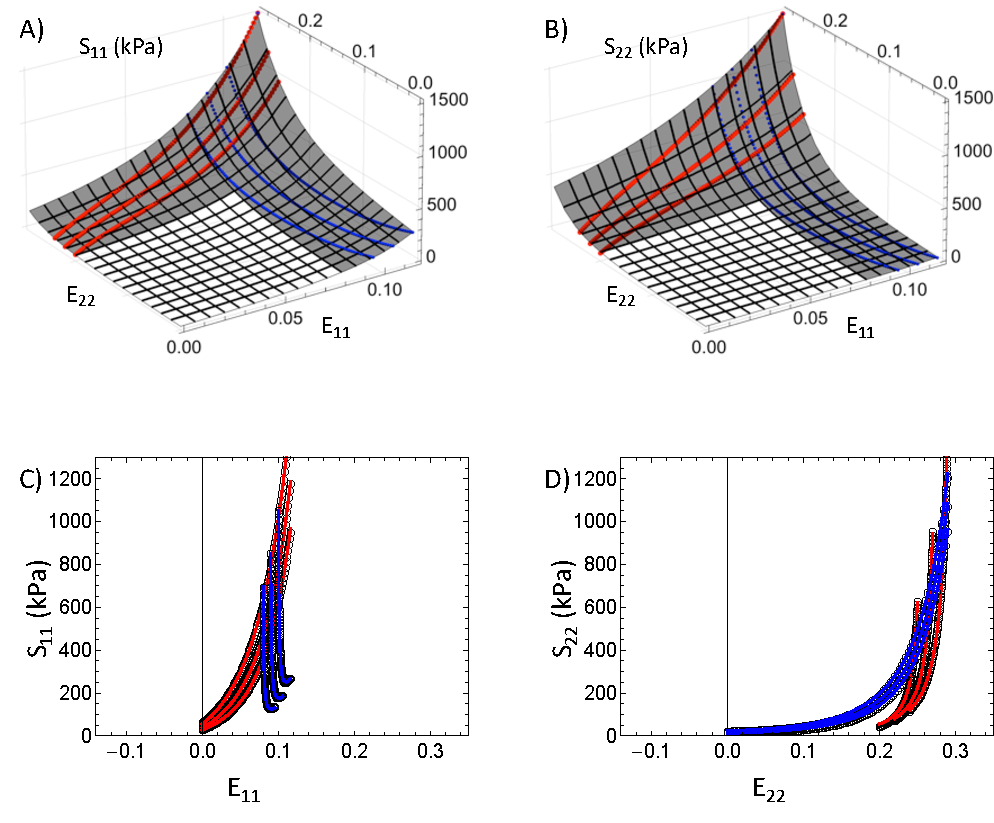
\includegraphics[width=6.5in]{Figures/effphyfit}
\caption{The fit of $\Psi_{eff}$ to the post-pre-strain loading paths is very good. A) The $S_{11}$ surface. B) The $S_{22}$ surface. C) Best fit of the $S_{11}$ component of the loading paths. D) Best fit of the $S_{22}$ component of the loading paths.}
\label{fig:effphyfit}
\end{figure} 
%-------------------	 end FIGURE 	-------------------%
%%%%%%%%%%%%%%%%%%%%%%%%%%%%%%%%%%%%%%%%%%%%%%%%%%%%%%%%%%%%

%%%%%%%%%%%%%%%%%%%%%%%%%%%%%%%%%%%%%%%%%%%%%%%%%%%%%%%%%%%%
%-------------------	begin FIGURE 	-------------------%
\begin{figure}[hptb]
\centering
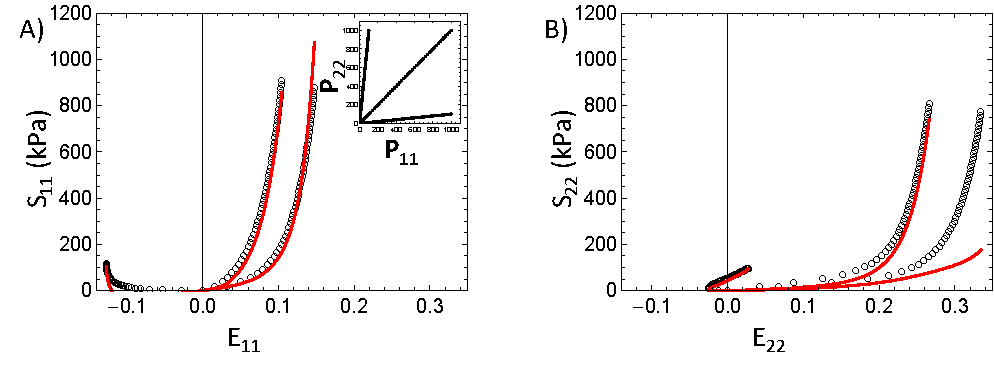
\includegraphics[width=6.5in]{Figures/effphypred}
\caption{$\Psi_{eff}$ predicts the A) $S_{11}$ component and B) $S_{22}$ component of the unfitted loading paths very poorly even though the fit to the post-pre-strain range is very good (Fig. \ref{fig:effphyfit}). The inset in A shows the corresponding loading paths.}
\label{fig:effphypred}
\end{figure} 
%-------------------	 end FIGURE 	-------------------%
%%%%%%%%%%%%%%%%%%%%%%%%%%%%%%%%%%%%%%%%%%%%%%%%%%%%%%%%%%%%


	

%%%%%%%%%%%%%%%%%%%%%%%%%%%%%%%%%%%%%%%%%%%%%%%%%%%%%%%%%%%%
%-------------------	begin FIGURE 	-------------------%
\begin{figure}[hptb]
\centering
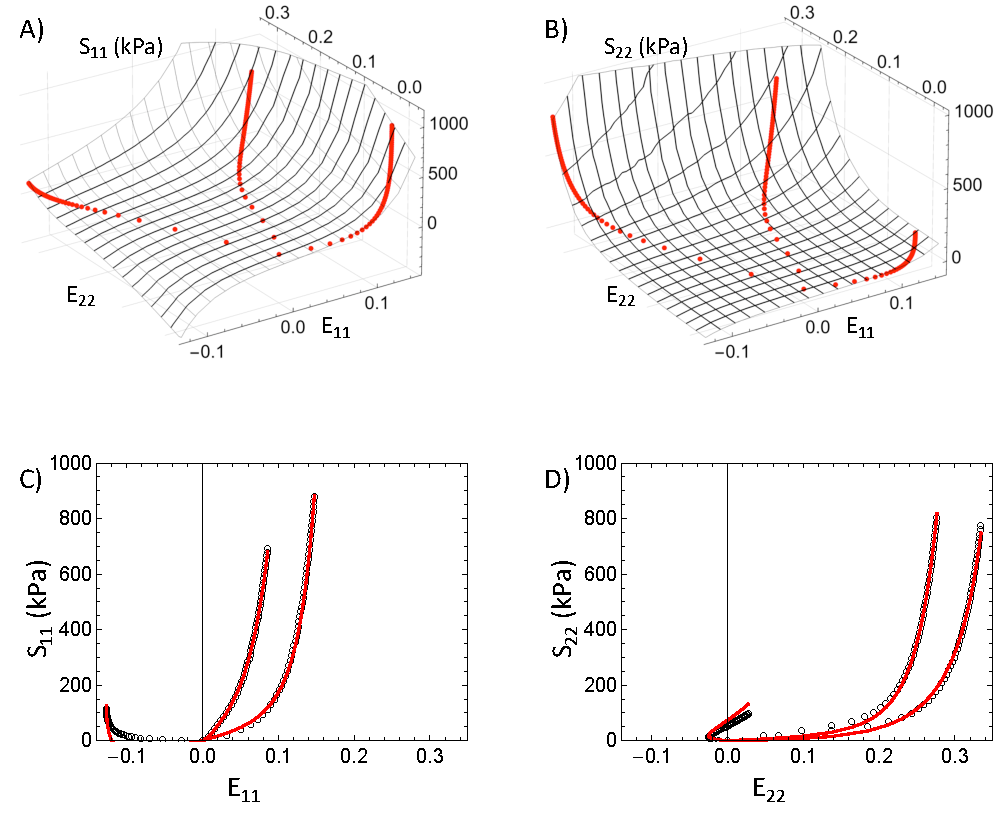
\includegraphics[width=6.5in]{Figures/effoptfit}
\caption{$\Psi_{eff}$ fit optimal loading paths very well. A) The $S_{11}$ surface. B) The $S_{22}$ surface. C) Best fit of the $S_{11}$ component of the loading paths. D) Best fit of the $S_{22}$ component of the loading paths.}
\label{fig:effoptfit}
\end{figure} 
%-------------------	 end FIGURE 	-------------------%
%%%%%%%%%%%%%%%%%%%%%%%%%%%%%%%%%%%%%%%%%%%%%%%%%%%%%%%%%%%%

%%%%%%%%%%%%%%%%%%%%%%%%%%%%%%%%%%%%%%%%%%%%%%%%%%%%%%%%%%%%
%-------------------	begin FIGURE 	-------------------%
\begin{figure}[hptb]
\centering
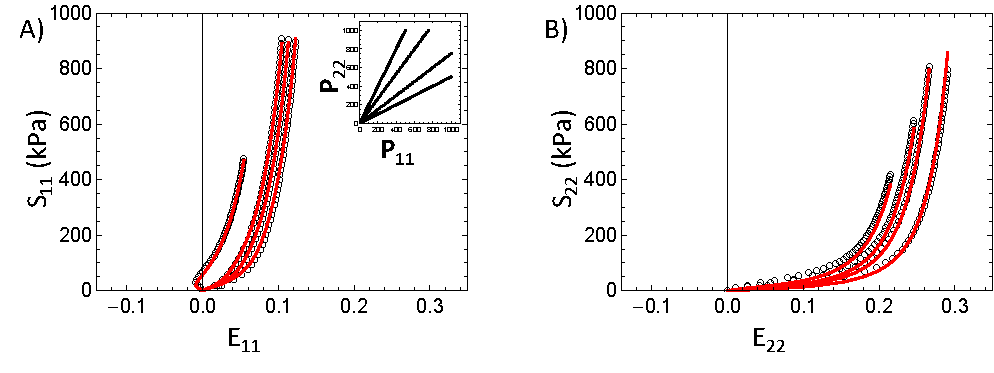
\includegraphics[width=6.5in]{Figures/effoptpred}
\caption{Combining $\Psi_{eff}$ with optimal loading paths to predicts the A) $S_{11}$ component and B) $S_{22}$ component of the remaining unfitted loading paths very well from fit (Fig. \ref{fig:effoptfit}). The inset in B shows the corresponding loading predicted paths.}
\label{fig:effoptpred}
\end{figure} 
%-------------------	 end FIGURE 	-------------------%
%%%%%%%%%%%%%%%%%%%%%%%%%%%%%%%%%%%%%%%%%%%%%%%%%%%%%%%%%%%%





	



%-----------------------------------------------------------
%	Simulation
%-----------------------------------------------------------
\subsection{Numerical simulation of equibiaxial tension process for the BHV leaflet tissues}
	
    Planar biaxial test simulations were conducted to ensure that $\Psi_{eff}$ (Eqn. \ref{eqn:finalexponentialmodelformscaled}) and the elasticity tensor (Appendix \ref{sec:elasticitytensor}, Eqn. \ref{eqn:greenelasticityform}) were properly implemented in the finite element simulation framework. The results matched perfectly (Fig. \ref{fig:biaxvalidation}). We compared the computation time for both the $\Psi_{eff}$ and the Holzapfel-Gasser-Ogden model for biaxial simulation of BHV tissues and expectedly found no significant increase in computational cost. The total elapsed time for $\Psi_{eff}$ is 7.58 seconds in comparison to 6.40 seconds for the Holzapfel-Gasser-Ogden model, much faster than any micro-models can achieve.  

	Next we simulated tri-leaflet valves with model parameters derived from bovine pericardium, porcine aortic valve leaflet, and an idealized isotropic case. This is a simple demonstration of the use of the $\Psi_{eff}$ for the upscaling and homogenizing of micro-models. The model parameters for the bovine pericardium case was derived from the simplified structural model and model parameter of Aggarwal and Sacks \cite{aggarwal_inverse_2015}, and the resulting response matched very well qualitatively. Due to a lack of fiber mapping in the quasi-static simulation software used, some minor difference are still expected. We found no difficulty when simulating the pericardium, aortic, or isotropic valves. Suggesting that $\Psi_{eff}$ is quite robust numerically. 

\begin{figure}
\centering
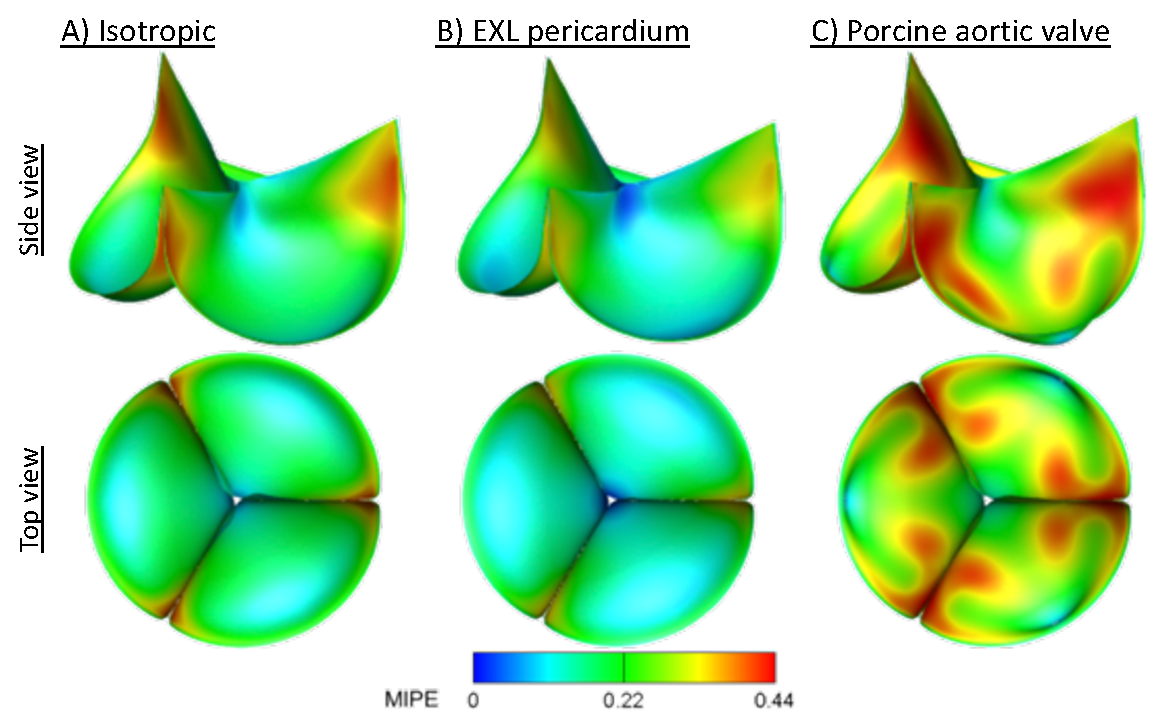
\includegraphics[width=6.5in]{Figures/valvesimulations}
\caption{Simulations of intact tri-leaflet valves using A) the porcine aortic valve properties with an isotropic fiber orientation distribution, B) exogenously cross-linked bovine pericardium properties with the most homogenous stress distribution, and C) the porcine aortic valve properties properties which results in a very heterogeneous stress distribution and the belly region caving in. The top row shows the side view of the valves at 80 mmHg and the bottom row shows the top-down view of the valves at the same transvalvular pressure.}
\label{fig:valvesimulations}
\end{figure}
    
    The material property has significant effects on the mechanical behaviors of the leaflets (Fig. \ref{fig:valvesimulations}). The results are plotted with the maximum in plane Green-Lagrange strain (MIP$\mathbf{E}$). When comparing the three different material, we can see that the native aortic valve properties results in significant heterogeneities in the deformation of the leaflets (Fig. \ref{fig:valvesimulations}C). Specifically, the belly region of the leaflets significantly protrudes out, increasing the load in the surrounding regions, especially near the commissures. This results in some stress concentrations that are not conducive to heart valve durability and health in general. The bovine pericardium valve (Fig. \ref{fig:valvesimulations}B) and the isotropic valve (Fig. \ref{fig:valvesimulations}A) on the other hand has significantly more homogeneous leaflet deformations, especially from the top-down view. Both of these undergoes approximately the same deformation of 0.2 in MIPE. The largest difference between the two is near the commissure regions of the valve. Where the isotropic case is under significantly higher strain. Functionally, the material properties of the exogenously cross-linked bovine pericardium is the most suitable for the valve leaflets, where it more evenly distribute the stresses. 
    
    Much of the reasons behind these differences is likely to be due to the differences between the apparent mechanical properties \textit{in vivo} and the measured mechanical response in the laboratory setting. This is especially true for the properties aortic valve, which is extremely anisotropic with very high compliance in the radial direction of the leaflets. This difference is most likely due to the mismatch of referential configuration between the two state. Residual strain or residual stress has significant impact on the functional properties of the leaflets, specifically the apparent anisotropy and stiffness. Collagen fiber directions and varying regional properties can also have significant impact on the functional properties of the leaflets, and thus the results of the simulation. The valve leaflet shape, root geometry and properties, the arterial or ventricular geometry and loading conditions, can all be significant factors affecting the functions of the valves and in distributing the stress in the leaflets. Furthermore, how these factors affect the fluid dynamics of the valves is also an interesting question, suitable for further study. All in all, this is meant to be a demonstration and proof of concept for using $\Psi_{eff}$ to handle a wide range of soft tissue behaviors and anisotropy for the simulation of biological organs, in this case heart valves. Further and more detailed studies will be reserved for the future.  
  
     
%	To further validate the model, we tested its utility in numerical simulations. Using the Finite Element framework developed by Hsu \textit{et al.}, we implemented the effective constitutive model for simulating tri-leaflet valves. We utilized the heart valve geometry and boundary conditions in Aggarwal and Sacks \cite{aggarwal_inverse_2015} and approximated the effective constitutive model parameters to simulate the quasi-static loading of an intact heart valve. The results are qualitatively compared to those of Aggarwal and Sacks \cite{aggarwal_inverse_2015} for validation.







%\begin{figure}
%\centering
%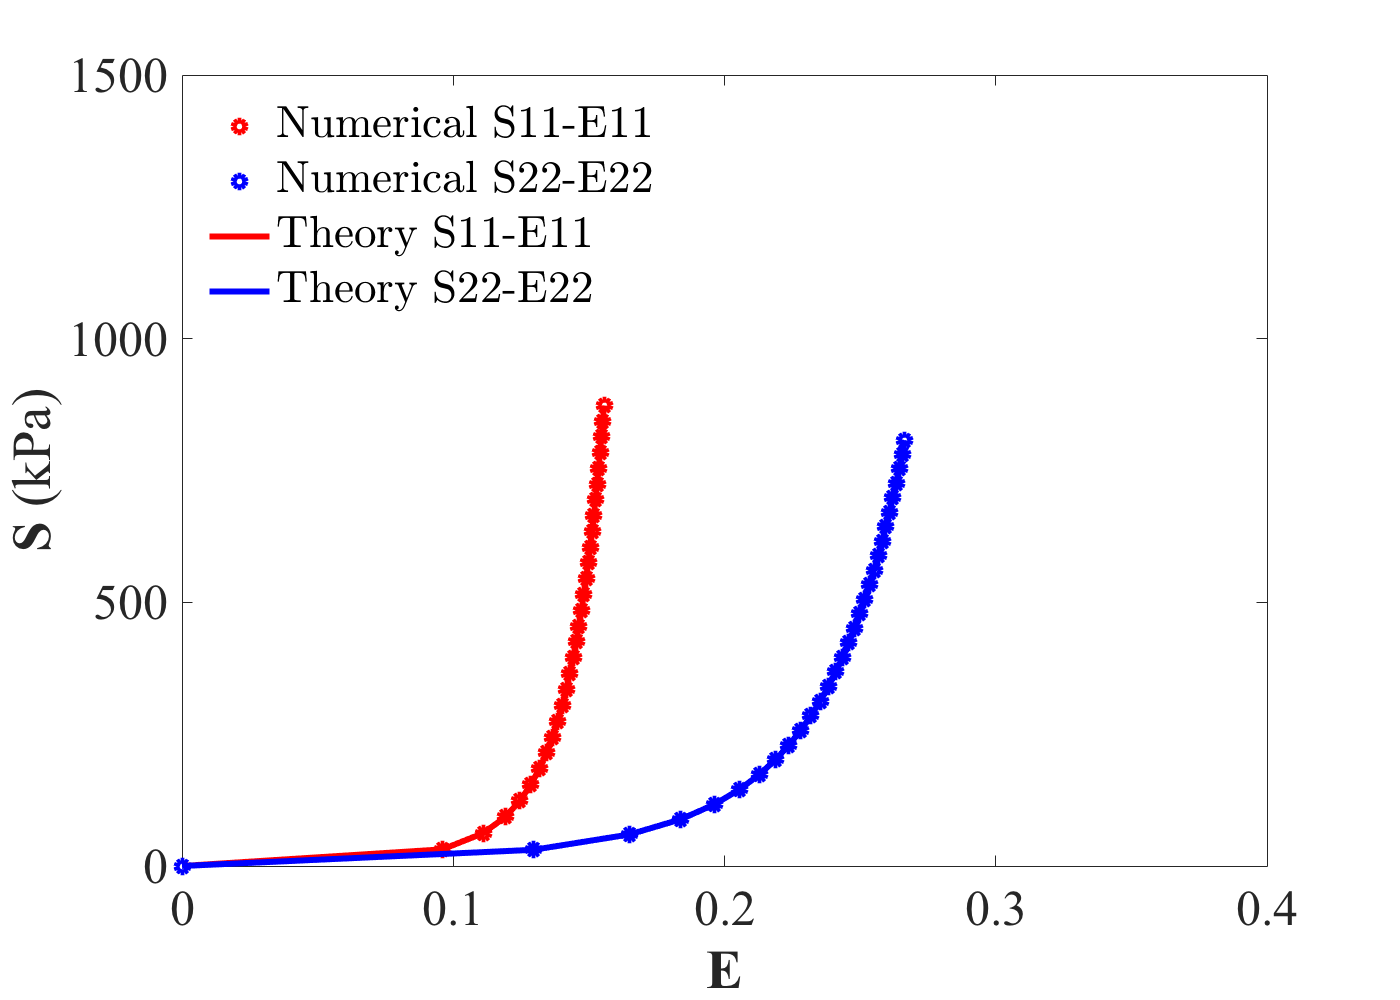
\includegraphics[width=5in]{Figures/validation.png}
%\label{fig:validation}
%\end{figure} 




    



    
    
    
    
    
    
    
    
    
    
    
    
    
    
    

